\chapter{Literature Review of Fault Localization in Computer Networks Using
End-to-End Measurements}

This chapter briefly describes three projects (Argus, NetNorad and CEM)
that deploy end-to-end measurements to localize faults in computer networks.

\section{Argus}

In
~\cite{argus_end_to_end_service_anomaly_detection_and_localization_from_an_isps_point_of_view}
is presented Argus, a system to
detect and localize QoS issues in ISP's networks. To achieve this goal, it uses
end-to-end data and network global information, such as
traffic passively monitored at end-users, the ISP network topology,
routing tables, and geographic information. Argus's infrastructure is defined by
the pipeline presented in figure ~\ref{fig:argus_pipeline}.

\begin{figure}[H]
    \centering
    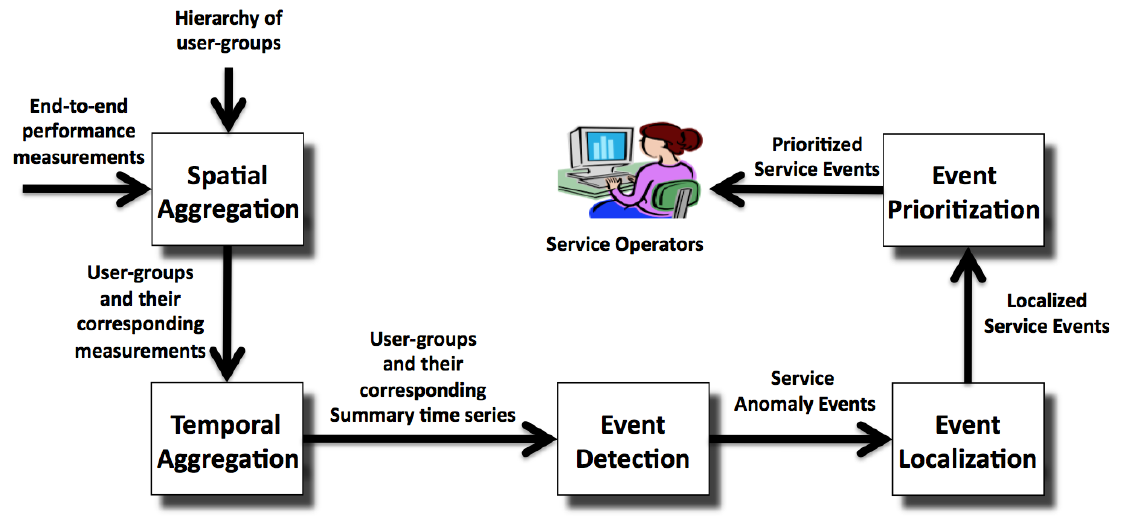
\includegraphics[width=1.0\textwidth]{./figures/literature_review/argus_pipeline.png}
    \caption{Argus pipeline.}
    \label{fig:argus_pipeline}
\end{figure}%

The system operation starts with the spatial aggregation procedure, in which
end-users are clustered into user-groups. This step avoids keeping
track of the end-to-end performance metrics associated with lots of
individual end-users, which improves the system's scalability.
Each user-group is characterized by a set of end-users that share some common
attributes, such as BGP prefix or AS. The used attributes imposes the possible
fault locations to be infered.
An example of a spatial agreggation is presented in figure
~\ref{fig:argus_spatial_aggregation}.

\begin{figure}[H]
    \centering
    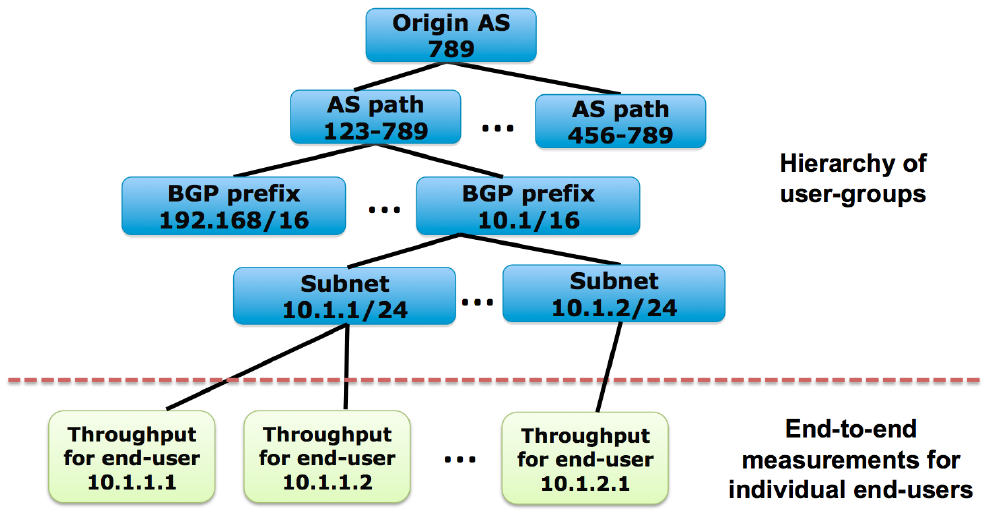
\includegraphics[width=1.0\textwidth]{./figures/literature_review/argus_spatial_aggregation.png}
    \caption{Argus spatial aggregation.}
    \label{fig:argus_spatial_aggregation}
\end{figure}%

The temporal aggregation phase determines how the performance metrics
from different end-users of an end-group are combined.
For each user-group the
measurements of all end-users are grouped by time-bins, and for each
time-bin a summary statistic, such as median or mean, is selected.
Each type of fault can be better tracked by a specific statistic.
As an example, the
minimum of the RTT's measurements can capture the physical propagation delay,
while the average can be associated with network congestion. Argus uses median
as the default transformation, since it was empirically identified as
effective to track network problems, and also robust to individual
end-users variability caused by their local infrastructure.

The event detection procedure applies algorithms to detect anomalies in the
summary time series. Argus uses a Holt-Winters variation,  which consists of
an online
method with low runtime and memory complexities, essential qualities to a
scalable system.

The responsability of the event localization step is to infer fault locations
using spatial and events times correlations.
However, the detailed description of how this
process is implemented was not published.

Finally, after the problem localization, the events are sorted according with
their
significance. During the ranking, the method considers metrics obtained
through the event detection
algorithm, and also the number of end-users affected by the events.

Argus was evaluated using RTT measurements of a CDN hosted in a tier-1 ISP.
During an
one month period with time-bins of 1 hour, Argus detected 2909
anomaly events. In general, lower level user-groups were more responsible
for those events than the higher level groups,
and only a small fraction of the end-users affected the end-group anomaly.
Also, 90\% of the events lasted for
at most 1 hour, which was the used time-bin granularity.

Although not analysed through the Argus paper, the fact that only a small number
of end-users are responsible for the end-groups events, is an indication that
fault localization can achieve higher precision if spatial aggregation is
applied with finer granularity.

TALK ABOUT GRCA

\section{NetNorad}

NetNorad ~\cite{netnorad} consists of a Facebook's internal project to
automate the analysis of faults in the Facebook's
network. Previous techniques face several disadvantages, for instance,
human-driven investigation may take hours. Also, cases known as gray failures
cannot be detected only collecting devices information through SNMP or command
line
interface. For example, some devices cannot report it's own malfunctioning, or
some issues can be related with the global network stucture.

Facebook's network is structured hierarchically. At the
lowest level there are servers in hacks, which are organized in
clusters. A set of clusters in the same building and attached to
the same network characterize a data center. Data centers are grouped
through a network that interconnects them within the same region, and appends
to the Facebook global backbone. Figure
~\ref{fig:netnorad_network_architecture} presents an example of this
architecture.

\begin{figure}[H]
    \centering
    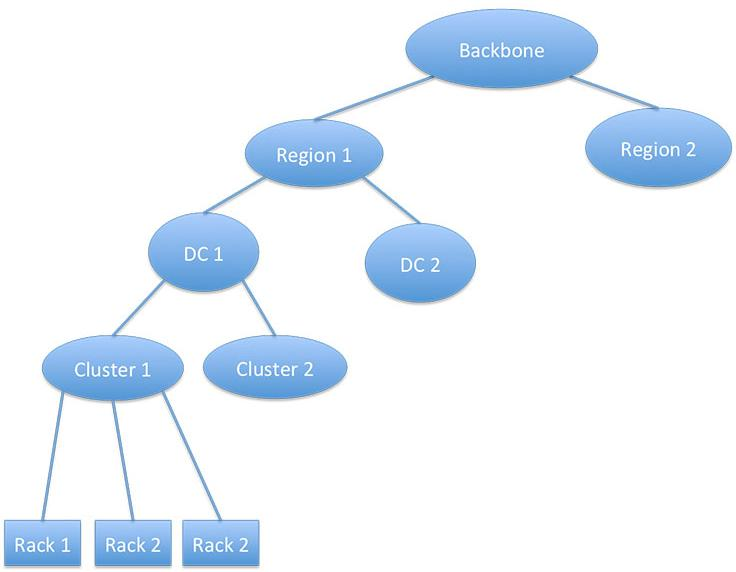
\includegraphics[width=1.0\textwidth]{./figures/literature_review/netnorad_network_architecture.jpg}
    \caption{Facebook's network architecture.}
    \label{fig:netnorad_network_architecture}
\end{figure}%

NetNorad is mainly based on loss and RTT end-to-end measurements.
Facebook's servers ping each other, in which
a pinger sends UDP packets to responders, and the latter
send the packets back. The process happens in turns, in which each pinger
sends packets to all targets, collects the responses, and then repeats
the procedure.

A small number of pingers are placed in each cluster, and the responders are
deployed on all machines. All pingers share a target list, which includes
at least two machines of every rack.
As with Argus, NetNorad applies spatial aggregation techniques.
The pingers group the responses of machines that belong to the same cluster
during a round, and tags them according with their location.
Tags are defined by the following patterns:
"DC" if the target cluster is in the same data center of the pinger;
"Region" if the target cluster is outside the
data center but within the same region;
"Global" if the target cluster is outside the pinger's
region.

With the tagging process, each cluster have three time series reflecting
different spatial viewpoints. Then, the system tracks
distinct percentiles over 10-minute
intervals, which enables the isolation of
network events. For instance, a packet loss spike at the
50th percentile means that probably there is a failure affecting the majority of
machines, while a peak at the 90th and not at 50th
percentile can indicate a small fraction of anomalous servers.
For each combination of proximity tag and percentile is defined two
thresholds, one for trigger and another for clear an alarm.

Considering the three tags, if a high loss is detected in a cluster,
then the fault is probably located at the cluster's data center.
Also, if all clusters in a data center identify a QoS degradation,
then the fault is likely to be a layer above the clusters.
Although these simple reasonings can reduce the set of possible fault locations,
they are unable to exacly isolate them.
However, a Facebook tool called fbtracert,
can improve this analysis, exploring multiple
paths between two endpoints, and checking the
packet loss levels at every hop.

When automatic investigation is unable to find the failure, then there
is a human involvement to find it. A detailed accuracy analysis is not
presented, however, the infrastrucure allows alarms to be raised about 30
seconds far from the network events.

\section{CEM}

In ~\cite{crowdsourcing_service_level_network_event_monitoring} is proposed a
framework called Crowdsourcing Event Monitoring (CEM), in which a
monitoring software that runs inside or alongside applications is placed at the
end-hosts, enabling the detection of service-level events within seconds or
minutes.

In CEM, each end-host passively collects performance metrics related with a
specific service, such as a VOD application.
Through these data the end-host identifies local issues as
potential network events, and pushes them to a distributed storage to further
analysis.
The framework doesn't specifies how events should be detected,
however, they need to be associated with service-level problems.

Concurrent events ocurring in multiple
performance metrics of a service (e.g., download and upload rates), increases the
confidence that the problem is independent of the service.

The
fact that the events detection procedures are realized at the end-hosts
increases the scability of the system.

To spatially isolate network faults, multiple locally detected events are
centrally correlated.
The first considered subproblem in this step is to check if concurrent events
are caused by a
network fault. There are several reasons to different hosts experiences
concurrent events. One is the target of the work, which is a network fault.
Another one is that the service can experience a problem not caused by the
network, for example, a high volume of requests in a web service. Also it is
possible that concurrent events occur only by chance, for example, users
experience interference on separate wireless routers. To solve this problem the
framework provides a statistical model to determine if
concurrently events are a coincidence or not. This model takes in
consideration service-specific dependencies and the rate of observed local
events ocurring at the same the same time in a network. In this model, the
confidence in a detected event being due to a network increases with the
number of hosts detecting the event, and with the increase of independent
performance metrics indicating the event. To isolate the problem the framework
uses structure information about the network and the hosts geographic
locations, however, ther work doesn't provides any details of how this
correlation is made.

CEM was deployed and evaluated in a P2P system, using BitTorrent traces collected
from users of the Ono plugin for the Vuze BitTorrent client. The detected
events by the system was compared to aground truth
of network events gathered from public available event reports of ISPs.

The following inferences are not presented in the paper.
CEM provides a high level framework structure, however lack for several details
in the deployment procedure.
